\section{Præsentation af spil, evaluering af krav og perspektivering}

\begin{frame}{Spil præsentation}
\begin{columns}
	\begin{column}{.49\textwidth}
	\centering
		\begin{figure}[H]
   			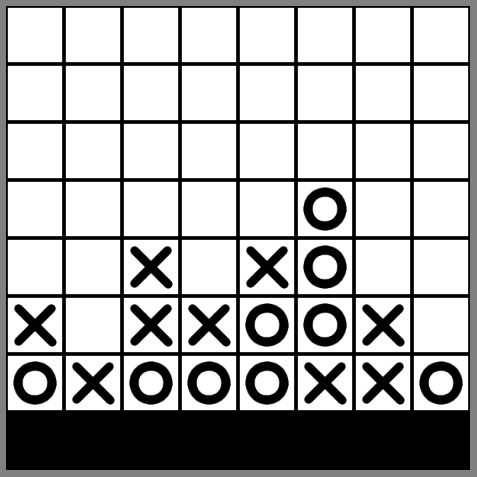
\includegraphics[scale=0.18]{billeder/connect4.png}
   			\caption{Connect four}
		\end{figure}
	\hspace{0.3cm}
	\centering
		\begin{figure}[H]
   			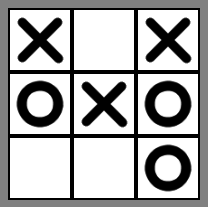
\includegraphics[scale=0.28]{billeder/noughtncrosses.png}
   			\caption{Kryds og bolle}
		\end{figure}
	\end{column}
	\hfill
	\begin{column}{.49\textwidth}
		\begin{figure}[H]
   			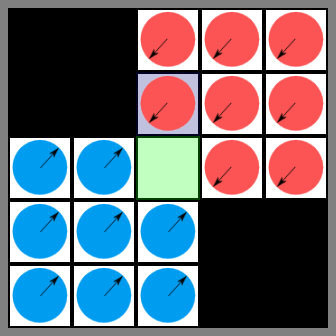
\includegraphics[scale=0.23]{billeder/kentspil.png}
   			\caption{Kents spil}
		\end{figure}
		\begin{figure}[H]
   			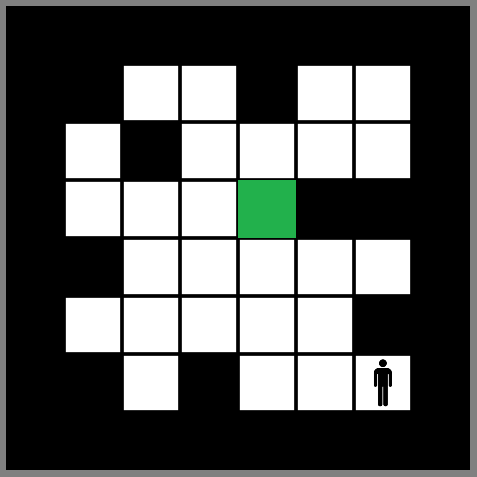
\includegraphics[scale=0.18]{billeder/ice.png}
   			\caption{Ice}
		\end{figure}
	\end{column}
\end{columns}
\end{frame}

\begin{frame}{Connect four}
 	\begin{figure}
    	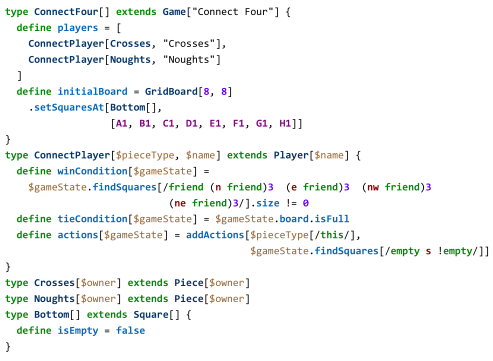
\includegraphics[width=0.8\linewidth]{billeder/connect4_codeexample.png}
 	\end{figure}
\end{frame}

\begin{frame}{Evaluering af krav}
	\begin{itemize}
		\item Programmeringssproget kan bruges til at programmere brætspil i
		\item Det skal være muligt at implementere skak inklusiv dets specielle regler
		\item Det skal være muligt at lave brætspil på relativt få linjers kode
		\item Junta brætspil skal kunne spilles i en simulator
	\end{itemize}	
\end{frame}

\begin{frame}{Evaluering af krav}
	\begin{itemize}
		\item Det skal være muligt at spille spillene over netværk
		\item Programmeringssproget må ikke være en udvidelse af et eksisterende programmeringssprog 
		\item Brætspillene skal være spilbare på forskellige platforme
	\end{itemize}	
\end{frame}

\begin{frame}{Perspektivering}
  \vspace{0.5cm}
  \begin{itemize}
		\item Tilfældige værdier
		\vspace{0.1cm}
		\item Et stærkere action-system
	\end{itemize}
	\begin{figure}[H]
   			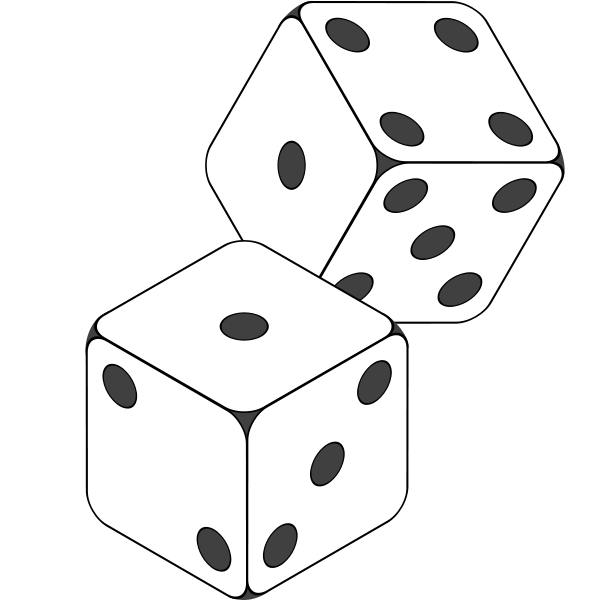
\includegraphics[scale=0.15]{billeder/2-Dice-Icon.png}
	\end{figure}	
\end{frame}

\begin{frame}{Perspektivering}
	\vspace{0.4cm}
	\begin{itemize}
		\item Forskellige brættyper
	\end{itemize}
	\begin{figure}[H]
   		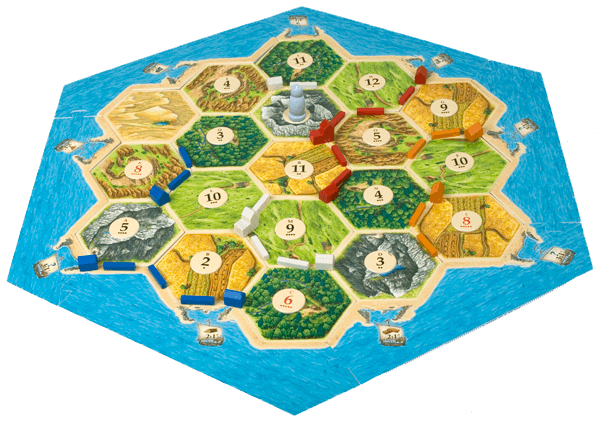
\includegraphics[scale=0.3]{billeder/settlers-board2.png}
	\end{figure}	
\end{frame}